\chapter{Introdução}

\section{Contexto}

Medir a qualidade do código-fonte  de um software é um processo fundamental no seu desenvolvimento, pois daí surgem indicadores sobre os efeitos que uma alteração no código irá causar ou sobre os efeitos gerados na qualidade do software após a adesão de uma nova prática na equipe de desenvolvimento \cite{Fenton98}. 

Através do processo de medição da qualidade interna do software é possível não só entender e controlar o que está se passando no seu desenvolvimento, como também ser encorajado a tomar decisões que visem a sua melhoria \cite{Fenton98}. Como a qualidade do código fonte está relacionada à qualidade interna do produto de software \cite{ISO25023}, sua medição, e consequentemente as melhorias implantadas nele melhoram a qualidade do produto como um todo. 
 

\section{Justificativa}

Buscando facilitar a interpretação das métricas de código fonte, bem como apoiar as decisões de refatoração a serem tomadas, \citeonline{rego_monitoramento_2014} elaborou um ambiente de \textit{Data Warehouse} para armazenamento de métricas, sobre o qual este trabalho irá analisar sua eficácia e eficiência no monitoramento da qualidade interna do software, sendo essa sua maior contribuição. Essa análise poderá ajudar equipes de desenvolvimento de software na escolha de uma maneira de aferir a qualidade interna do seu produto e tomar as decisões corretas sobre o que refatorar.

\section{Problema}
\label{intro_problema}

Apesar de métricas de código fonte serem coletadas facilmente através de ferramentas como o \textit{Sonar} e o \textit{Analizo}, sua interpretação ainda pode ser um desafio que se não for superado pode tornar essa coleta algo sem muito valor significativo. Ferramentas de análise de métricas frequentemente exportam seu resultado como valores numéricos isolados \cite{Meirelles2013} e números isolados a respeito do código não trazem consigo definições sobre o que deve ser refatorado. Surge a partir desse fato a necessidade de uma solução que apoie a tomada de decisão, associando esses valores numéricos a elementos mais fáceis de serem interpretados, como cenários de limpeza. 

Baseando-se no problema descrito e aproveitando a solução já desenvolvida, que utiliza um ambiente de \textit{Data Warehousing} para o monitoramento de métricas de código fonte, foi criada a seguinte questão geral de pesquisa:

\textbf{\textit{O uso de \textit{Data Warehousing} é eficaz e eficiente no monitoramento de métricas de código fonte, facilitando a interpretação dos resultados da análise estática e apoiando decisões de refatoração?} }

\section{Objetivos}

O objetivo geral deste trabalho consiste na análise da eficácia e eficiência do uso de \textit{Data Warehousing} no monitoramento de métricas de código fonte. Como este trabalho é dividido em duas partes, seus objetivos também foram divididos dessa forma, sendo os objetivos da primeira parte:

\begin{easylist}[itemize]	
	
	& Levantar fundamentação teórica que servirá de base para todo o trabalho.
	& Apresentar solução desenvolvida por \citeonline{rego_monitoramento_2014} para monitoramento de métricas através de \textit{Data Warehousing}. 
	& Elaborar o projeto do estudo de caso.
	
	\end{easylist}	

A segunda parte deste trabalho, a ser desenvolvida no primeiro semestre de 2015, terá os seguintes objetivos:	

\begin{easylist}[itemize]	
	
	& Coletar os dados que surgirão como respostas das questões específicas elaboradas para o estudo de caso, como por exemplo o nível de satisfação quanto ao uso da solução ou qual a taxa de oportunidade de melhoria de código em um determinado intervalo de tempo.
	& Realizar análise dos dados coletados.
	& Relatar resultados obtidos.
	
	\end{easylist}

\section{Metodologia de pesquisa}

Nessa seção será definida a metodologia da pesquisa, definindo qual a natureza da pesquisa, a forma de abordagem, o tipo de objetivo que se espera alcançar, os procedimentos técnicos e o tipo de coleta de dados. A figura \ref{fig:metodologiadepesquisa} apresenta um esquema para a metodologia, buscando classificar a pesquisa quanto aos elementos que a classificam segundo \citeonline{metodologia_edna}:

\begin{figure}[h!]
\centering
\includegraphics[keepaspectratio=false,scale=0.40]{figuras/figuras_matheus/metodologia_da_pequisa.eps}
\caption{Metodologia de pesquisa}
\label{fig:metodologiadepesquisa}
\end{figure}
\FloatBarrier

Do ponto de vista da natureza, uma pesquisa pode ser considerada básica ou aplicada \cite{metodologia_edna}. A pesquisa a qual esse trabalho se refere é aplicada pois seus resultados contém aplicação prática e são dirigidos à solução de problemas específicos.

A abordagem da pesquisa será tanto qualitativa quanto quantitativa, pois ao mesmo tempo em que busca classificar informações em números através de técnicas estatísticas, também analisa a subjetividade de algumas questões sem que isso seja traduzido em números.

O objetivo que essa pesquisa busca alcançar faz com que ela seja considerada descritiva, pois uma pesquisa descritiva visa descrever as características de determinado fenômeno envolvendo uso de técnicas padronizadas de coleta de dados \cite{metodologia_edna}. Quanto aos procedimentos técnicos ela pode ser considerada de levantamento, pois envolve a interrogação direta das pessoas cujo comportamento se deseja conhecer. Além disso, do ponto de vista dos procedimentos técnicos, ela também pode ser considerada bibliográfica, documental e como um estudo de caso.

Também foi modelado no esquema da metodologia quais serão as formas de coleta de dados. Como pode pode ser visto na figura \ref{fig:metodologiadepesquisa}, a coleta é feita através de questionários, obervação na vida real e documentos, que incluem o próprio relatório da solução adotada no estudo de caso.

Segundo \citeonline{wohlin2012experimentation} a condução de um estudo de caso deve obedecer os cinco passos listados de forma sequencial na figura \ref{fig:estudodecaso}: 

\begin{figure}[h!]
\centering
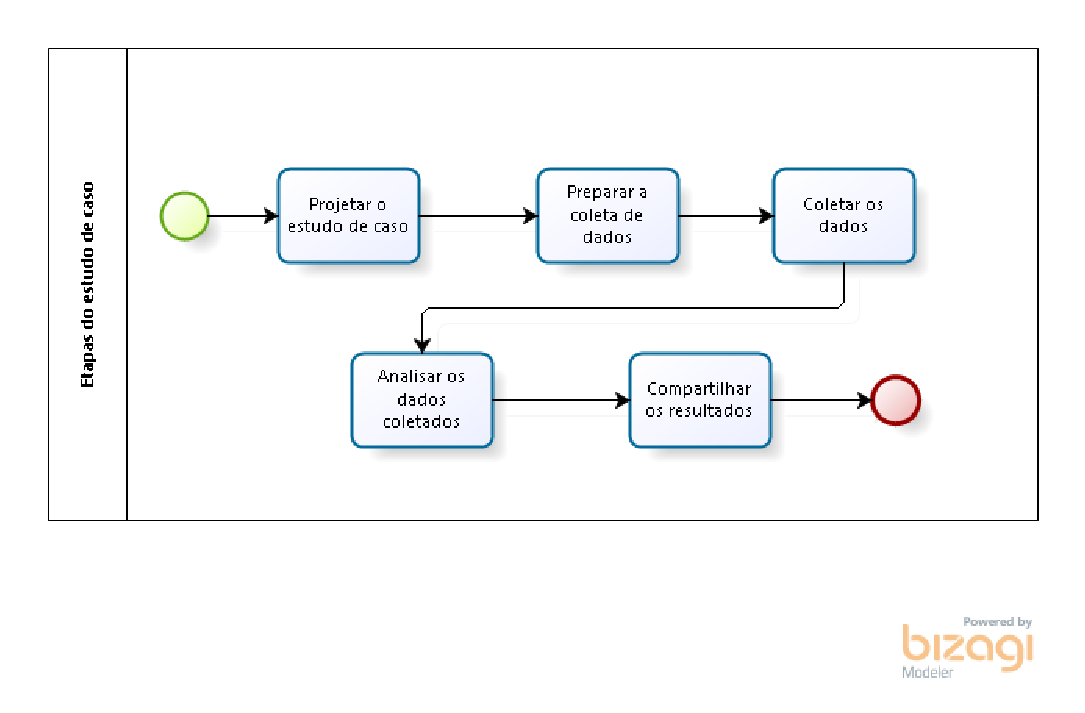
\includegraphics[keepaspectratio=false,scale=0.8]{figuras/figuras_matheus/estudodecaso.eps}
\caption{Estrutura do estudo de caso}
\label{fig:estudodecaso}
\end{figure}
\FloatBarrier

Projetar o estudo de caso e preparar a coleta de dados são etapas que consistem em uma macro atividade chamada de planejamento do estudo de caso. Nesse planejamento serão identificados elementos como o problema a ser resolvido e a questão de pesquisa a ser respondida, de modo que o protocolo de estudo de caso possa ser elaborado já determinando qual o método e a fonte da coleta dos dados. Coletar dados é uma atividade a ser executada em seguida, feita através de pesquisas bibliográficas e documentais além dos resultados extraídos da própria solução para monitoramento de código fonte a ser analisada durante o estudo de caso. Analisar os dados coletados diz respeito à interpretação dos dados coletados compreendendo não só análises quantitativas como também qualitativas. A etapa chamada de compartilhar os resultados, por sua vez, indica que os resultados coletados e interpretados são expostos neste trabalho a quem desejar fazer sua leitura. 


\section{Organização do Trabalho}

Este trabalho está dividido em 5 capítulos:

	\begin{easylist}[itemize]	
	
	& \textbf{Capítulo 1 - Introdução:} Esse capítulo tem como objetivo apresentar o contexto que esse trabalho está inserido, o problema sobre o qual ele buscará resolver, qual a justificativa e os objetivos da sua realização e como essa pequisa foi elaborada.
	& \textbf{Capítulo 2 - Métricas de Software:} Capítulo responsável pela explicação teórica a respeito do que são métricas de código e como elas foram utilizadas no desenvolvimento da solução que esse trabalho busca analisar.
	& \textbf{Capítulo 3 - Data Warehouse:} Nesse capítulo serão apresentados conceitos teóricos sobre \textit{Data Warehousing}, assim como a maneira como foi desenvolvido o ambiente de \textit{Data Warehouse} para armazenamento de métricas de código fonte.
	& \textbf{Capítulo 4 - Projeto de estudo de caso:} Será apresentada a estratégia de pesquisa adotada durante o trabalho, buscando elaborar um protocolo para o estudo de caso que será realizado. Elementos de pesquisa como o problema a ser resolvido, os objetivos a serem alcançados no estudo de caso e quais os métodos de coleta e análise dos dados serão identificados e explicados.
	& \textbf{Capítulo 5 - Conclusão:} Além das considerações finais dessa primeira parte do trabalho, serão descritos objetivos para a segunda parte a ser realizada ao término desta.
	
	\end{easylist}	
